% ---------- Titelblad Masterproef Faculteit Wetenschappen -----------
% Dit document is opgesteld voor compilatie met pdflatex.  Indien je
% wilt compileren met latex naar dvi/ps, dien je de figuren naar
% (e)ps-formaat om te zetten.
%                           -- december 2012
% -------------------------------------------------------------------
\RequirePackage{fix-cm}
\documentclass[12pt,a4paper,oneside]{article}

% --------------------- In te laden pakketten -----------------------
% Deze kan je eventueel toevoegen aan de pakketten die je al inlaadt
% als je dit titelblad integreert met de rest van thesis.
% -------------------------------------------------------------------
\usepackage{graphicx,xcolor,textpos}
\usepackage{helvet}

% -------------------- Pagina-instellingen --------------------------
% Indien je deze wijzigt, zal het titelblad ook wijzigen.  Dit dien je
% dan manueel aan te passen.
% --------------------------------------------------------------------

\topmargin -10mm
\textwidth 160truemm
\textheight 240truemm
\oddsidemargin 0mm
\evensidemargin 0mm

% ------------------- textpos-instellingen ---------------------------
% Enkele andere instellingen voor het voorblad.
% --------------------------------------------------------------------

\definecolor{green}{RGB}{172,196,0}
\definecolor{bluetitle}{RGB}{29,141,176}
\definecolor{blueaff}{RGB}{0,0,128}
\definecolor{blueline}{RGB}{82,189,236}
\setlength{\TPHorizModule}{1mm}
\setlength{\TPVertModule}{1mm}
%----------------------- Custom stuff -------------------------------
\graphicspath{./}
\usepackage{makeidx}
\index{hoofd}
\makeindex
\usepackage{amsmath}
\usepackage[english]{babel}
\usepackage{hyperref}
\usepackage[]{algorithm2e}
%------------------------ Plot packages ----------------------------
\usepackage{tikz}
\usepackage{pgfplots}
\usepackage{pgf}
\usepackage{units}
\usepackage{metalogo}
\usepackage{graphicx}
\usepackage{caption}
\usepackage{subcaption}

% ------------------------Meta data---------------------------------

\title{First Assignment Computational Methods for Astrophysical Applications}
\author{Vergauwen Bob}
\date{November 14, 2014}





\usepackage[style=verbose]{biblatex}

\usepackage{filecontents}% to embed the file `myreferences.bib` in your `.tex` file

\begin{filecontents}{myrefrences.bib}
@article{walker2011anderson,
  title={Anderson acceleration for fixed-point iterations},
  author={Walker, Homer F and Ni, Peng},
  journal={SIAM Journal on Numerical Analysis},
  volume={49},
  number={4},
  pages={1715--1735},
  year={2011},
  publisher={SIAM}
}
\end{filecontents}

\addbibresource{myreferences.bib}










\begin{document}
%title page
	\setbeamertemplate{headline}[title_page]
	\setbeamertemplate{footline}[title_page]
	\csname beamer@calculateheadfoot\endcsname %recalculate head and foot dimension
		\begin{frame}
			\titlepage
		\end{frame}
%head and foot for body text	
	\setbeamertemplate{headline}[body]
	\setbeamertemplate{footline}[body]

%%%%%%%%%%%%%%%%%%%%%%%%%%%%%%%%%%%%%%%%%%


\begin{frame}{Outline}
	\vskip 5mm
	\hfill	{\large \parbox{.95\textwidth}{\tableofcontents[hideallsubsections]}}
\end{frame}

\section{Introduction}
  \subsection{Euler equation for HD}
\begin{frame}{Introduction}
\begin{block}{Riemann problem in 2D}
	A Riemann problem consists of a system of conservation equation together with a piecewise constant initial condition.
\begin{tabular}{l l}
	\begin{minipage}{0.61\textwidth}
				\begin{equation*}
						U_t + F(U)_x + G(U)_y = 0
					\end{equation*}
					\begin{equation*}
						U_0(x,y) = 
						\begin{cases} u_1 & (x,y)  \in [0.5,1]^2 \\ 
						u_2 & (x,y)  \in [0,0.5]\times[0.5,1] \\ 
						u_3 & (x,y)  \in [0,0.5]^2 \\ 
						u_4 & (x,y)  \in [0.5,1]\times[0,0.5] \\ 
						\end{cases}
					\end{equation*}
	\end{minipage}
	&
	\begin{minipage}{0.4\textwidth}
	\hspace{10mm}
		\begin{figure}
			\centering
			\includegraphics[width=\textwidth]{../src2/figs/init.pdf}
		\end{figure}
	\end{minipage}
	\end{tabular}
	\end{block}
\end{frame}

\begin{frame}{The equations}

\begin{block}{Euler equation for compressible fluids}
\begin{equation*}
U_t + F(U)_x + G(U)_y = 0
\end{equation*}
with
\begin{equation*}
U =
 \begin{pmatrix}
 \rho \\
 \rho u \\
 \rho v \\
 e
 \end{pmatrix} \hspace{5 mm}
 F =
  \begin{pmatrix}
  \rho u\\
  \rho u^2 + p \\
  \rho u v\\
  u(e+p)
  \end{pmatrix} \hspace{5 mm}
   G =
    \begin{pmatrix}
    \rho v\\
    \rho u v \\
    \rho u^2 + p \\
    v(e+p)
    \end{pmatrix} \hspace{5 mm}
\end{equation*}
Equation describing the dynamics of a compressible fluid.
Conserved quantities are: $ \rho $ density, $ \rho u $ momentum in $ x $ , $ \rho v$ momentum in $ y $ and the total energy $ e $.
\end{block}

\end{frame}




  
\section{Numerical schemes}
  \subsection{Overview of different numerical methods}
\begin{frame}{Numerical methods}

5 different numerical schemes tested:
\begin{itemize}
  	\item TVDLF
  	\item  HLL
  	\item HLLC
  	\item TVD-MUSCL 
  	\item FD
\end{itemize}

\end{frame}


\begin{frame}{TVDLF}
content...
\end{frame}

\begin{frame}{TVD-MUSCL}
content...
\end{frame}

\begin{frame}{HHL and HLLC}
content...
\end{frame}

\begin{frame}{FD}
content...
\end{frame}

\section{Software and computations}
  \subsection{Software and computations}

\begin{frame}{MPI-AMRVAC and the HPC}


\begin{figure}
\centering
\includegraphics[width=0.7\linewidth]{../../figs/vsc}
\label{fig:vsc}
\end{figure}

\end{frame}


\begin{frame}{Server interaction}

A script can do this better than we do!

\begin{itemize}
\item No need to ssh
\item All changes can be made locally 
\item Bulk submitting
\item No need to wait on the compilation
\item Compresses and downloads all automatic
\end{itemize}

Les then 10 minutes to compare 5 methods on a new problem.
\end{frame}

\begin{frame}{Some problems}
\vspace{2cm}
\begin{itemize}
\item Compiler error: segmentation problem
\item Some of the problems ran only on one node 
\item The visualisation software crashed a lot
\end{itemize}

\end{frame}
 \section{Numerical results}
 \section{Results}

In this section we briefly give some results and explain our findings.
We used the standard functions for $ P,Q $ and $ \rho $.
If we used a positive sign for $ g $ no roots existed, this is the case there is a heavier fluid on top of a lighter one and was not stable.
The function calculated for the positive values for $ g $ blew up exponentially.

\subsection{Dispersion relations}

\subsubsection{Dispersion of $ K^2 $}
As a first experiment conducted we held all parameters fixed, ($ \sigma = 1, g = -1 $ ) except for the value of $ K^2 $.
For this parameters we than searched for the eigenvalues for several modes.
This yields dispersion curves of the allowed values for $ \omega $ as a function of $ K^2 $ as given in Figure \ref{fig:DispersionRelations}.
The result in this plot looks very similar to what is given in the assignment.


\subsubsection{Dispersion of $ \sigma^2 $}
Next we calculated the dispersion relation for $ \sigma^2 $. All the other parameters where again held constant $ (g = -1,K^2 = 1) $.
The result of this is given in Figure \ref{fig:DispersionRelations}.
The shape of the curves look very similar as the dispersion for $ K $, but the value for omega drops rapidly if we search for higher order solutions.


\subsubsection{Dispersion of $ g $}
The final dispersion relation we investigated was the one of $ g $ and $ \omega^2 $.
This is given in Figure \ref{fig:DispersionRelations}.
Surprisingly there looks like a linear relation between $ g $ and $ \omega^2 $, this is completely different from the previous two dispersion relations.

\begin{figure}[h!]
        \centering
        \begin{subfigure}[b]{0.49\textwidth}
                \includegraphics[width=9cm]{../src/plot/DispersionK}
\caption{The dispersion relation of $ K $ and $ \omega $. The line at the top is for the firs mode, the green line underneath is for the second mode and so on. }
                \label{fig:gull}
        \end{subfigure}%
        ~ %add desired spacing between images, e. g. ~, \quad, \qquad, \hfill etc.
          %(or a blank line to force the subfigure onto a new line)
        \begin{subfigure}[b]{0.49\textwidth}
                \includegraphics[width=9cm]{../src/plot/DispersionSigma}
\caption{The dispersion relation of $ \sigma $ and $ \omega $. The line at the top is for the firs mode, the green line underneath is for the second mode and so on.}
                \label{fig:tiger}
        \end{subfigure}\\
        
        ~ %add desired spacing between images, e. g. ~, \quad, \qquad, \hfill etc.
          %(or a blank line to force the subfigure onto a new line)
        \begin{subfigure}[b]{.5\textwidth}
                 \includegraphics[width=9cm]{../src/plot/DispersionG}
\caption{The dispersion relation of $ g $ and $ \omega $. The line at the top is for the firs mode, the green line underneath is for the second mode and so on.}
                \label{fig:mouse}
        \end{subfigure}
        \caption{Several dispersion relations for the various variables and modes of the equation.}\label{fig:DispersionRelations}
\end{figure}
 \subsection{2D Riemann problem}
 \subsection{Results Part A}


\begin{frame}{Configuration 1 - Results from paper}	
\begin{figure}
\centering
\includegraphics[width=0.8\linewidth]{../../figs/configuration1_paper}
\label{fig:configuration1_paper}
\end{figure}
\end{frame}

\begin{frame}{Configuration 1 - Own results}
	movie
\end{frame}

\begin{frame}{Configuration 5 - Results from paper}	
	
\begin{figure}
\centering
\includegraphics[width=0.6\linewidth]{../../figs/configuration5_paper_1}
\label{fig:configuration5_paper_1}
\end{figure}

\begin{figure}
\centering
\includegraphics[width=0.5\linewidth]{../../figs/configuration5_paper_2}
\label{fig:configuration5_paper_2}
\end{figure}

\end{frame}

\begin{frame}{Configuration 5 - Own results}
	movie
\end{frame}

\begin{frame}{Configuration 5 - Own results}
	High Resolution - HLLC
	
\begin{figure}
\centering
\includegraphics[width=0.7\linewidth]{../../figs/Configuration5_HighRes}
\label{fig:Configuration5_HighRes}
\end{figure}

\end{frame}
	
  \subsection{Explosion}
 
\begin{frame}{Setup for the explosion}	

We tried several parameters
\begin{itemize}
\item Size of the explosion centre
\item Pressure difference 
\item Location of the explosion
\end{itemize}
\vspace{1cm}
        	  	\begin{minipage}{0.3\textwidth}
        	  	\begin{block}{}
        	  				\vspace{-1.7cm}
        	  	     	  	\begin{figure}
        	  	     	  	      	  \centering
        	  	     	  	      	  \includegraphics[width=\textwidth]{../../figs/exp/circ}
        	  	     	  	 \end{figure}
        	  	\end{block}
        	  	\end{minipage}
        	  	\begin{minipage}{0.3\textwidth}
        	  			\begin{block}{}
        	  			\vspace{-1.7cm}
        	  				\begin{figure}
        	  						\centering
        	  						\includegraphics[width=\textwidth]{../../figs/exp/sqr}
        	  					\end{figure}
        	  		  	\end{block}
        	  	\end{minipage}
				\begin{minipage}{0.3\textwidth}
        	  			\begin{block}{}
        	  			\vspace{-1.7cm}
        	  				\begin{figure}
        	  						\centering
        	  						\includegraphics[width=\textwidth]{../../figs/exp/corner}
        	  					\end{figure}
        	  		  	\end{block}
        	  	\end{minipage}
\end{frame}

\begin{frame}{Comparing two explosions}

Play the movie

\end{frame}

\begin{frame}{3d rayleigh taylor}



\end{frame}








	
  \subsection{3D Rayleigh–Taylor instabilities}
  \input{../LaTeX/resultsC.tex}
	\section{Conclusions}
	\input{../LaTeX/conclusions.tex}
  
 \end{document}
  
\section{Discrete systems}
  \begin{frame}{A three state system}
\begin{tabular}{l l}
	\begin{minipage}{0.61\textwidth}
		\begin{block}{Transition rates}
			\begin{equation*}
				\begin{cases}
				k(a,b)=e^{-\beta_1\epsilon}\\
				k(b,a)=1\\
				k(a,c) = 0\\
				k(c,a)=0\\
				k(b,c)=1\\
				k(c,b)=e^{-\beta_2\delta}\\
				\end{cases}
			\end{equation*}
		\end{block}
	\end{minipage}
	&
	\begin{minipage}{0.4\textwidth}
		\begin{figure}
			\centering
			\includegraphics[width=\textwidth]{../src/figure/Simple_3_State_System.pdf}
		\end{figure}
	\end{minipage}
	\end{tabular}
\end{frame}
% % % % % % % % % % % % % % % % % % % % % % % % % % % % % % % % % % % % % % % % %

  \subsection{analysic results}
  \begin{frame}{Analytic results: two transitions}
	\begin{tabular}{l l}
		\begin{minipage}{0.62\textwidth}
			\begin{equation*}
				\begin{cases}
					C_1 = \beta_1\epsilon e^{\beta_1\epsilon} \dfrac{\epsilon  + (\epsilon -\delta) e^{\beta_2\delta}}{T_1 \left( e^{\beta_1\epsilon} + 1 + e^{\beta_2\delta} \right)^2}\\
					\vspace{0pt}\\
					C_2 = \beta_2\delta e^{\beta_2\delta} \dfrac{\delta  + (\delta - \epsilon) e^{\beta_1\epsilon} }{T_2 \left( e^{\beta_1\epsilon} + 1 + e^{\beta_2\delta} \right)^2}
				\end{cases}
			\end{equation*}
			\begin{equation*}
				C_2 < 0 \Leftrightarrow \delta < \epsilon\dfrac{ e^{\beta_1\epsilon}}{1 + e^{\beta_1\epsilon} }
			\end{equation*}
			
		\end{minipage}
		&
		\begin{minipage}{0.38\textwidth}
			\vspace{-15pt}
			\begin{figure}
				\centering
				\includegraphics[height=0.44\textheight,keepaspectratio=true]{../src/plot/discreteSystems/C1InFunctionOfEpsilonAndDelta_1-eps-converted-to.pdf}
			\end{figure}
			\vspace{-25pt}
			\begin{figure}
				\centering
				\includegraphics[height=0.44\textheight,keepaspectratio=true]{../src/plot/discreteSystems/C2InFunctionOfEpsilonAndDelta_1-eps-converted-to.pdf}
			\end{figure}
		\end{minipage}
	\end{tabular}
\end{frame}
%%%%%%%%%%%%%%%%%%%%%%%%%%%%%%%%%%%%%%%%


\begin{frame}{Analytic results: three transitions}

	\begin{tabular}{l l}
		\begin{minipage}{0.62\textwidth}
			\begin{equation*}
				\begin{cases}
				C_1 = \dfrac{\epsilon\beta_1 e^{-\beta_1\epsilon} (e^{-\beta_1\epsilon}\epsilon+\epsilon+\delta)}
				{T_1(e^{-\beta_1\epsilon} + 2)^3 (e^{-\beta_2\delta} + 2)}\\
				\vspace{0pt}\\
				C_2 = \dfrac{\delta\beta_2 e^{-\beta_2\delta} (e^{-\beta_2\delta}\delta+\epsilon+\delta)}
				{T_2(e^{-\beta_1\epsilon} + 2) (e^{-\beta_2\delta} + 2)^3}
				\end{cases}
			\end{equation*}
		\end{minipage}
		&
		\begin{minipage}{0.38\textwidth}
			\vspace{-15pt}
			\begin{figure}
				\centering
				\includegraphics[height=0.44\textheight,keepaspectratio=true]{../src/plot/discreteSystems/C1InFunctionOfEpsilonAndDelta_2-eps-converted-to.pdf}
			\end{figure}
			\vspace{-25pt}
			\begin{figure}
				\centering
				\includegraphics[height=0.44\textheight,keepaspectratio=true]{../src/plot/discreteSystems/C2InFunctionOfEpsilonAndDelta_2-eps-converted-to.pdf}
			\end{figure}
		\end{minipage}
	\end{tabular}

\end{frame}

  \subsection{Simulations}
	\begin{frame}{Simulation of discrete system}
  Two methods have been used to simulate the discrete system.
  \begin{tabular}{l l}
  	\begin{minipage}{0.5\textwidth}
  		\begin{block}{Deterministic methode}
		\begin{itemize}
		\item Uses the Markov framework
		\item Transition matrix
		\item Fast
		\item Easy to implement
		\item No direct physics involved, just mathematics
		\item Can be speed up by linearisation
		\end{itemize}
  		\end{block}
  	\end{minipage}
  	\begin{minipage}{0.5\textwidth}
  			\begin{block}{ Stochastic methode}
  				\begin{itemize}
  				  \item Uses the a jump process
  				  \item The outcome is random
  				  \item One jump at the time
  				  \item Slow
  				  \item Represents the physical system very good
  				  \item Can produce more stochastic information
  				\end{itemize}
  		  	\end{block}
  	\end{minipage}
  	\end{tabular}
\end{frame}
\begin{frame}{Deterministic method}
\vspace{-1.5cm}
    	\begin{tabular}{l l}
    	  	\begin{minipage}{0.5\textwidth}
    	  	\begin{block}{Algorithme }
    	  	     	  		\begin{itemize}
    	  	     	  		\item Create  a transition matrix  $M(T)$
    	  	     	  		\item Chose an initial distribution  $\rho_0$
    	  	     	  		\item Update the distribution  $ \rho(t) = \rho_0 e^{Mt}$
    	  	     	  		\item Calculate the energy $E$
    	  	     	  		\item Change the temperature by a small fraction
    	  	     	  		\item repeat this process
    	  	     	 \end{itemize}
    	  	\end{block}
    	  	\end{minipage}
    	  	\begin{minipage}{0.6\textwidth}
    	  			\begin{block}{}
    	  				\begin{figure}
    	  						\centering
    	  						\includegraphics[width=\textwidth]{../src/plot/discreteSystems/TotalEnergyFunctionOfT2.pdf}
    	  					\end{figure}
    	  		  	\end{block}
    	  	\end{minipage}
    	  	\end{tabular}	
    	
\end{frame}

\begin{frame}{Stochastic method}
  \vspace{-1.5cm}
      	\begin{tabular}{l l}
      	  	\begin{minipage}{0.5\textwidth}
      	  	\begin{block}{Algorithme }
      	  	     	  		\begin{itemize}
      	  	     	  		\item Pick a random starting position
      	  	     	  		\item Let the particle jump for some steps
      	  	     	  		\item Calculate the energy
      	  	     	  		\item Repeat this for a good result
      	  	     	  		\item Change the temperature by a small fraction
      	  	     	  		\item repeat this process
      	  	     	 \end{itemize}
      	  	\end{block}
      	  	\end{minipage}
      	  	\begin{minipage}{0.6\textwidth}
      	  			\begin{block}{}
      	  				\begin{figure}
      	  						\centering
      	  						\includegraphics[width=\textwidth]{../src/plot/discreteSystems/TotalEnergyFunctionOfT2Stochastic.pdf}
      	  					\end{figure}
      	  		  	\end{block}
      	  	\end{minipage}
      	  	\end{tabular}	
      	
\end{frame}

\begin{frame}{Comparison of the two results}

     \vspace{1cm}
     
      	  	\begin{minipage}{0.49\textwidth}
      	  	\begin{block}{Two transitions }
      	  				\vspace{-1.7cm}
      	  	     	  	\begin{figure}
      	  	     	  	      	  \centering
      	  	     	  	      	  \includegraphics[width=\textwidth]{../src/plot/discreteSystems/AllInOneFixedTemp.pdf}
      	  	     	  	 \end{figure}
      	  	\end{block}
      	  	\end{minipage}
      	  	\begin{minipage}{0.49\textwidth}
      	  			\begin{block}{Three transitions}
      	  			\vspace{-1.7cm}
      	  				\begin{figure}
      	  						\centering
      	  						\includegraphics[width=\textwidth]{../src/plot/discreteSystems/AllInOneFixedTemp3transitions.pdf}
      	  					\end{figure}
      	  		  	\end{block}
      	  	\end{minipage}

      	
\end{frame}
\section{Continuous system}
  \begin{frame}{Langevin dynamics}
	\vspace{-12pt}
		\tikzstyle{every picture}+=[remember picture]
		\tikzstyle{na} = [baseline=-.5ex]
		\begin{equation*}
			\ddot{x} =  
			\tikz[baseline]{\node[fill=blue!20,anchor=base] (t1){$F$};} 
			-
			\tikz[baseline]{\node[fill=red!20,anchor=base] (t2){$\nabla U$};}
			-
			\tikz[baseline]{\node[fill=green!20,anchor=base] (t3){$\gamma \dot{x}$};}
			+
			\tikz[baseline]{\node[fill=orange!20,anchor=base] (t4){$\sqrt{2T\gamma}\xi_t$};}
		\end{equation*}
	\begin{tabular}{l l}
	\begin{minipage}{.85\textwidth}
		\begin{itemize}
			\item constant force $ F $ \tikz[na]\node [coordinate] (n1) {}; 
			\item force caused by periodic potential  \tikz[na]\node [coordinate] (n2) {};$U$
			\item friction, proportional to the velocity \tikz[na]\node [coordinate] (n3) {};
			\item Brownian motion \tikz[na]\node [coordinate] (n4) {};
		\end{itemize}
		\begin{tikzpicture}[overlay]
			\path[->]<1-> (n1) edge [bend right] (t1);
			\path[->]<1-> (n2) edge [out= 95, in=-70] (t2);
			\path[->]<1-> (n3) edge [out=0, in=-30] (t3);
			\path[->]<1-> (n4) edge [out=-20, in=-50] (t4);
		\end{tikzpicture}
	\end{minipage}
	\begin{minipage}{0.16\textwidth}
		\flushleft
		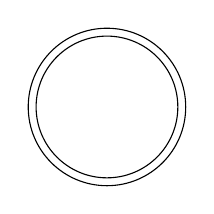
\begin{tikzpicture}
			\draw (0,0) circle (1cm)
						circle (.9cm);
		\end{tikzpicture}
	\end{minipage}
	\end{tabular}
	\begin{tabular}{l l}
		\begin{minipage}{0.5\textwidth}
			\vspace{-1.9cm}
			\begin{block}{Underdamped}
				Particle needs infinite time to reach its final velocity
			\end{block}
		\end{minipage}
		&
		\begin{minipage}{0.5\textwidth}
			\vspace{-.3cm}
			\begin{block}{Overdamped}
				Very high friction\\
				$ \rightarrow $ particle instantaneously reaches its final velocity $ v_f $
				\vspace{-5pt}
				\begin{equation*}
				\gamma v_f = F - \nabla U + \sqrt{2T\gamma}\xi_t
				\end{equation*}
			\end{block}
		\end{minipage}
	\end{tabular}
\end{frame}




  \subsection{Analytic results}
    \begin{frame}{The Fokker-Planck equation}
	\vspace{-5pt}
	\begin{equation*}
		\frac{\partial \mu_t (x)}{\partial t} + \nabla j_{\mu_t}(x) = 0, \hspace{15pt}  j_{\mu_t} = \frac{1}{\gamma}\mu_t \left( F - \nabla U \right) - \frac{\nabla\mu_t}{\beta\gamma}
	\end{equation*}
	\vspace{-10pt}
	\begin{block}{Solution}
		\begin{itemize}
			\item  \fbox{$F = 0$}  $ \rightarrow $  equilibrium \hspace{12pt} $\rho(x)=\dfrac{1}{\mathcal{Z}} e^{-\beta U(x)}, \hspace{5pt} \mathcal{Z} = \int_{0}^{1} e^{-\beta U} \dif x $
			\item  \fbox{$F\neq 0$}  and $ \int_{0}^{1}F \dif x \neq 0 $ $ \rightarrow $ no equilibrium
			\begin{equation*}
				\rho (x)= \frac{1}{\mathcal{Z}}\int_{0}^{1} \beta\gamma e^{\beta W(y,x)} \dif y, \hspace{15pt}
				\mathcal{Z} = \int_{0}^{1} \int_{0}^{1} \beta\gamma e^{\beta W(y,x)} \dif y \dif x
			\end{equation*}
			\begin{equation*}
				W(y,x) = U(y) - U(x) +
				\begin{cases}
					\int_{y}^{x}F \dif z  \hspace{5pt} &\text{ for } y\leq x\\
					\int_{y}^{1}F \dif z + \int_{0}^{x}F\dif z \hspace{5pt} &\text{ for } y>x
				\end{cases}
			\end{equation*}
		\end{itemize}
	\end{block}
\end{frame}

\begin{frame}{The Fokker-Planck equation}
	\begin{figure}
		\centering
		\includegraphics[width=.8\textwidth]{../src/plot/langevin/RhoInFunctionOfX_Langevin-eps-converted-to.pdf}
		\caption{$\rho(T)$ with $U= \sin(4\pi x)$, $k_b=1$, $\gamma=1$}
	\end{figure}	
\end{frame}
  \subsection{Simulations}
  	\begin{frame}{Simulation of the Langevin equation}
Two possible approximation methods.
  		\begin{block}{Overdamped}
  	  		\begin{equation*}
  	  		\dot{v} = F - \nabla U - \gamma v + \sqrt{2T\gamma}\xi_t
  	  		\end{equation*}
  	  	\end{block}
  	  	\begin{itemize}
  	  	 \item This is the most general method
  	  	\end{itemize}
  	  	\begin{block}{ Underdamped}
  	  		  			\begin{equation*}\label{eqn:overdamped}
  	  		  			\gamma v_f = F - \nabla U + \sqrt{2T\gamma}\xi_t
  	  		  			\end{equation*}
  	  		  			\begin{itemize}
  	  		  			\item Particle reaches terminal velocity after each step
  	  		  			\end{itemize}
  	  	\end{block}
\end{frame}


\begin{frame}{Results}
The result for both methods gave the same numerical result.
  \vspace{0cm}
       
        	  	\begin{minipage}{0.49\textwidth}
        	  	\begin{block}{}
        	  				\vspace{-1.7cm}
        	  	     	  	\begin{figure}
        	  	     	  	      	  \centering
        	  	     	  	      	  \includegraphics[width=\textwidth]{../src/plot/langevin/workOverTimeInFunctionOfTimePotential2.pdf}
        	  	     	  	 \end{figure}
        	  	\end{block}
        	  	\end{minipage}
        	  	\begin{minipage}{0.49\textwidth}
        	  			\begin{block}{}
        	  			\vspace{-1.7cm}
        	  				\begin{figure}
        	  						\centering
        	  						\includegraphics[width=\textwidth]{../src/plot/langevin/workInFunctionOfTimeUnerDamped.pdf}
        	  					\end{figure}
        	  		  	\end{block}
        	  	\end{minipage}
        	  	
\end{frame}

\section{Conclusion}
\subsection{analysic results}
  \input{../LaTeX/conclusions.tex}
  \section*{}
 



\begin{frame}
\vspace{3cm}
	\begin{minipage}[b]{.9\linewidth}
	\epigraph{``The best thing about learning about equilibrium, is that nothing changes" }{Anonymous}
		
	\end{minipage}
\end{frame}

\end{document}
